\documentclass{article}
\usepackage{amsmath,mathtools}
\usepackage{amssymb}
\usepackage{xargs}
\usepackage[dvipsnames]{xcolor}
\usepackage[margin=1.2in]{geometry}
\usepackage{graphicx}
\usepackage{enumitem}
\usepackage{pgfplots, pgfplotstable}
\usetikzlibrary{arrows.meta,bending,datavisualization.formats.functions,decorations.markings,decorations.pathmorphing}
\usepgfplotslibrary{fillbetween}
\usetikzlibrary{patterns}
\usepackage{tikz}

\begin{document}

% \begin{center}
%   \begin{tikzpicture}
%       \begin{axis}[
%         ylabel=$y$,
%         xlabel=$z$,
%         xmin=-.5,xmax=2.2,
%         ymin=-.5,ymax=1.5,
%         legend pos=outer north east,
%         axis lines=center,
%         legend style={legend cell align=right,legend plot pos=right}]

%       \addplot[dashed, color=blue,domain=-0.5:2.2,samples=100] {1};
%       \addplot[dashed, color=blue,domain=-0.5:2.2,samples=100,forget plot] {0};
%       \addlegendentry{$0\le y\le1$}
%       \addplot[dashed, color=red,domain=-0.5:2.2,samples=100] {x-1};
%       \addplot[dashed, color=red,domain=-0.5:2.2,samples=100,forget plot] {x};
%       \addlegendentry{$y\le z\le y+1$}

%       \plot[name path=G1, thick,samples=100,domain=-0.5:2.2,
%         forget plot,draw=none] {x-1};
%       \plot[name path=G2,thick,samples=100,domain=-0.5:2.2,
%         forget plot,draw=none] {x};
%       \addplot[fill=red,
%         % opacity=.8,
%         pattern=horizontal lines,
%         pattern color=red]
%         fill between [of=G1 and G2, soft clip={domain=-0.5:2.2}];

%       \plot[name path=B1, thick,samples=100,domain=-0.5:2.2,
%         forget plot,draw=none] {1};
%       \plot[name path=B2,thick,samples=100,domain=-0.5:2.2,
%         forget plot,draw=none] {0};
%       \addplot[fill=blue,
%         % opacity=.8,
%         pattern=vertical lines,
%         pattern color=blue]
%         fill between [of=B1 and B2, soft clip={domain=-0.5:2.2}];
%       \end{axis}
%   \end{tikzpicture}
%   \end{center}

% \begin{center}
%   \begin{tikzpicture}
%       \begin{axis}[
%         xlabel=$z$,
%         xmin=-.5,xmax=1,
%         ymin=-.5,ymax=1,
%         legend pos=outer north east,
%         axis lines=center,
%         legend style={legend cell align=right,legend plot pos=right}]

%       \addplot[dashed, color=red,domain=-0.5:2.2,samples=100] {2*x};
%       \addlegendentry{$f(z)$}

%       \end{axis}
%   \end{tikzpicture}
%   \end{center}

\begin{center}
  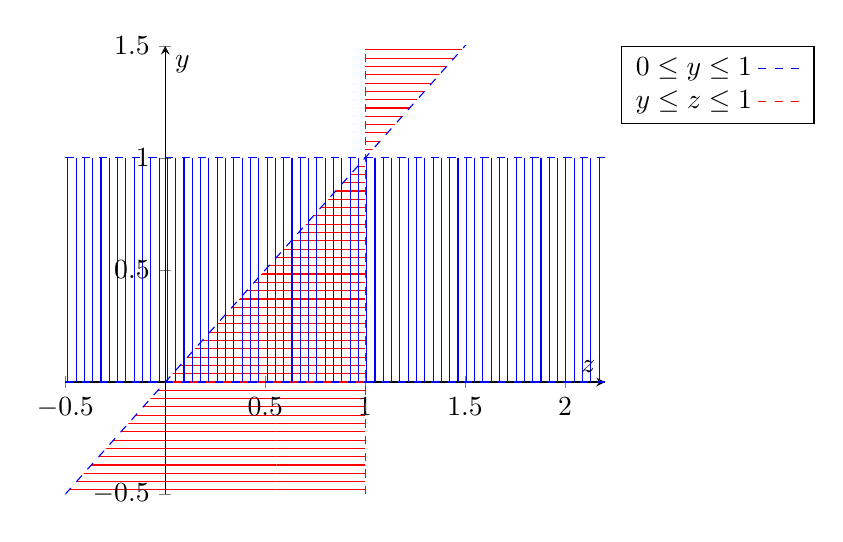
\begin{tikzpicture}
      \begin{axis}[
        ylabel=$y$,
        xlabel=$z$,
        xmin=-.5,xmax=2.2,
        ymin=-.5,ymax=1.5,
        legend pos=outer north east,
        axis lines=center,
        legend style={legend cell align=right,legend plot pos=right}]

      \addplot[dashed, color=blue,domain=-0.5:2.2,samples=100] {1};
      \addplot[dashed, color=blue,domain=-0.5:2.2,samples=100,forget plot] {0};
      \addlegendentry{$0\le y\le1$}
      \addplot +[name path=G1, mark=none,dashed, color=red,] coordinates {(1, -.5) (1, 1.5)};
      \addplot[name path=G2,dashed, color=blue,domain=-0.5:2.2,samples=100,forget plot] {x};
      \addlegendentry{$y\le z\le 1$}

      \addplot[fill=red,
        % opacity=.8,
        pattern=horizontal lines,
        pattern color=red]
        fill between [of=G1 and G2, soft clip={domain=-0.5:2.2}];

      \plot[name path=B1, thick,samples=100,domain=-0.5:2.2,
        forget plot,draw=none] {1};
      \plot[name path=B2,thick,samples=100,domain=-0.5:2.2,
        forget plot,draw=none] {0};
      \addplot[fill=blue,
        % opacity=.8,
        pattern=vertical lines,
        pattern color=blue]
        fill between [of=B1 and B2, soft clip={domain=-0.5:2.2}];
      \end{axis}
  \end{tikzpicture}
  \end{center}

\end{document}